\section{Introduction}

% 1. explain constancy and in particular size constancy

Consider \figref{fig1}. Humans can effortlessly perceive two chairs of roughly the same height and tell that one is much closer than the other, though still further away than the person, who is taller than the chairs. Compare this to what a state-of-the-art object detector tells us about the image: that there are two chairs, 120 and 40 pixels tall, and one person with 200 pixels from top to bottom. How can we enable computer vision systems to move beyond this crude 2D representation and allow them to capture richer models of their environments, such as those that humans take for granted?

The 3D world is a lot more structured than it looks like from the retina (or from a camera sensor), where objects jump around with each saccade and grow and shrink as we move closer or farther from them. We do not perceive any of this because our brains have learned priors about how visual inputs correlate with the underlying environment, and this allows us to directly access realistic and rich models of scenes. The priors we use can be categorized as being related to either \textit{geometry} or \textit{familiarity}.

\begin{figure}[t!]
  \centering
  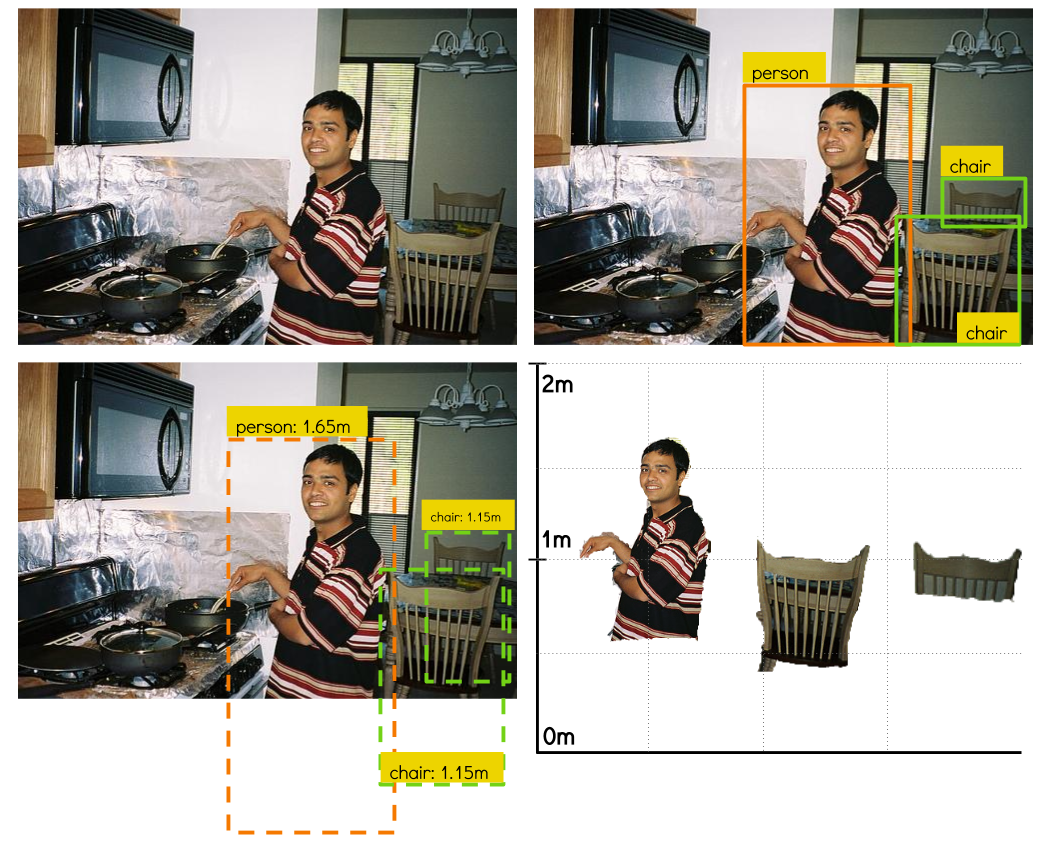
\includegraphics[width=\textwidth]{figures/amodal/Fig_1.png} % COCO_train2014_000000352357.jpg
%  \includegraphics[width=0.22\textwidth]{figures/amodal/coco_occlusions}
  \caption{\figlabel{fig1} Perceiving the veridical size of objects in realistic scenes, from a single image, requires disentangling size and depth, being able to compensate for occlusions and to determine intrinsic camera parameters. We tackle all three of these problems, leveraging recent developments in object recognition and large annotated object and scene datasets.}
\end{figure}

Image projection properties, such as the fact that the distance of an object from the camera dictates apparent size and that parallel lines in the scene vanish in the image, provide useful signal for perceiving structure. Familiarity cues are complementary and impose expectations on individual objects and configurations -- we expect most objects to be supported by another surface and we have the notion of \textit{familiar size} -- similar objects are of similar sizes. In this work, we exploit geometry and familiarity cues and develop a framework to build richer models of the visual input than those given by current computer vision systems, which are still largely confined to the 2D image plane.

The notion that certain geometrical cues can aid perception has been known since the time of Euclid - the points in the image where objects touch the ground together with their perceived heights allows inference of real world object size ratios \cite{burton45}. Familiarity cues, on the other hand must be learned, which can be done using available annotations and building upon rapid recent progress in object recognition, more robustly harnessed to explain novel images. Similar ideas have been proposed by Hoiem \etal~\cite{hoiem2008putting,Hoiem:book} and Gupta \etal ~\cite{gupta2010blocks} who studied the interaction between object detection and scene layout estimation and showed that, by reasoning over object sizes within their 3D environment, as opposed to within the image, one could perform better object detection. Lalonde \etal~\cite{lalonde2007photo} and Russell \etal~\cite{russell2009building} also tackled a problem similar to operationalizing size constancy and inferred object sizes of annotated objects. These works, while sharing similar goals to ours, were limited in their scope as they assumed fully visible instances - object recognition technology at the time being a limiting factor. In this paper, we aim for veridical size estimation in more realistic settings -- where occlusions are the rule rather than the exception. Occlusions present a significant technical challenge as they break down a number of assumptions(\eg in 
\figref{fig1} not modeling occlusions would yield an incorrect estimate of the relative depths of the two chairs shown).

To overcome these challenges, we first introduce amodal completion. This is a very well studied ability of human perception, primarily in the context of amodal edge perception \cite{kanizsa1979organization}, building on theories of \textit{good continuation} \cite{shipley2001fragments}. In the context of objects, amodal completion manifests itself as inference of the complete shape of the object despite visual evidence for only parts of it \cite{breckon2005amodal}.
%Psychology: Do Artists See Their Retinas? Cavanagh
%Amodal completion: Amodal volume completion: 3D visual completion. Fisher
%Organization in vision: Essays on Gestalt perception. Kanizsa 1979
In \secref{amodalCompletion}, we tackle the amodal completion task and frame it as a recognition problem, formalized as  predicting the full extent of object bounding boxes in an image, as opposed to only the visible extent. We build amodal extent predictors based on convolutional neural networks which we train on the challenging PASCAL VOC dataset. In \secref{sizeconstancy}, we propose a formulation that, leveraging amodally completed objects, can disentangle relative object sizes and object distances to the camera. This geometric reasoning allows us only to infer distances for objects up to a scaling ambiguity in each image. To overcome this ambiguity, we show in \secref{sceneFocal} that it is possible to leverage statistical dependencies between scenes and intrinsic camera parameters, and learn to predict focal lengths of scenes from large scale scene datasets. Finally, we present qualitative  results exhibiting veridical size estimation in complex scenes.

%The 3D world is a lot less wild than it looks like from the retina or from a camera sensor. In the retina, due to saccades, objects jump around several times per second. They also grow as we get closer, and get smaller as we move away. The ability to factor out such artifacts of seeing from the true nature of the scenes being seen is called \textit{visual constancy} and makes possible a more seamless interaction of an agent with its environment.


%Computer vision systems are still largely confined to the image plane. For example, in fig. \ref{fig1}, a state-of-the-art object detector localizes three people having heights of 100, 70 and 140 pixels, instead of three people of approximately the same height. Support relationships provide important cues for size constancy by leveraging time-proven Euclidean geometry: the points in the image where objects touch the ground together with their perceived heights allows inference of real world object size ratios \cite{}. Another important cue is familiarity (recognition). As an example, face sizes vary within a narrow range, so their dimensions in the image are informative of nearness to the camera.

%[Say something about size from familiarity (recognition)]

%Both types of cues are affected by occlusions, which translate into depth distortions, but have not yet been considered in prior art \cite{}. In this paper we tackle the size constancy problem in more generality, in realistic settings -- where occlusions are the rule rather than the exception -- by introducing amodal completion. We introduce amodal completion predictors based on convolutional networks which we train on especially engineered datasets having both natural and synthetic occlusion patterns. Additionally, we propose a formulation that, leveraging amodal completion, can disentangle relative class sizes and object distances to the camera from  training data having just ground truth bounding boxes and class labels. Finally, we present qualitative detection results exhibiting size constancy in complex Microsoft COCO scenes. 


